%%%% This CV has been greatly influence by
%%%% the extended fancy cv from Carmine Benedetto.
%%%% I thank him for the excellent work. Unfortunately 
%%%% it wouldn't compile on my machine. So I worked it out myself.

\documentclass{article} 
\usepackage[ngerman]{babel}% deutsche Trennregeln
\usepackage{microtype}% verbesserter Randausgleich
\usepackage[utf8]{inputenc}
\usepackage{graphicx}
\usepackage{color}
\usepackage{xcolor}
\usepackage[obeyspaces]{url} 
\usepackage[left=0.5cm,top=0.25cm,right=0.5cm,bottom=0.5cm,nohead,nofoot]{geometry}

\usepackage{fontawesome}
%https://www.wolframalpha.com/input/?i=seismic+magnitude
\usepackage{svg}

\makeatletter
\setlength{\@fptop}{40pt}
\makeatother

\usepackage{pdfcomment}
% Fix incorrect display of tooltips (http://tex.stackexchange.com/a/74340/3323)
\makeatletter
\renewcommand{\pc@annot@tooltip}%
{%
  /TU (\pc@pdfenc@contents)\space%
  /T (tooltip \thezref@unique)\space%
  /C [0 0 0]\space%
  /FT/Btn\space%
  /Ff 65536\space%
  /H/N\space%
}%

  
\definecolor{white}{RGB}{255,255,255}
\definecolor{anti-flashwhite}{rgb}{0.95, 0.95, 0.96}

\definecolor{darkgray}{HTML}{333333}
\definecolor{gray}{HTML}{4D4D4D}
\definecolor{lightgray}{HTML}{999999}

\definecolor{green}{HTML}{C2E15F}
\definecolor{orange}{HTML}{FDA333}
\definecolor{purple}{HTML}{D3A4F9}
\definecolor{red}{HTML}{FB4485}
\definecolor{blue}{HTML}{6CE0F1}
\definecolor{pblue}{HTML}{0395DE}

\usepackage[framemethod=tikz]{mdframed}
\usepackage{tikz}
\newcommand*{\ClipSep}{0.4cm}%


\usepackage{hyperref}
\hypersetup{
    pdftitle={},
    pdfauthor={},
    pdfsubject={},
    pdfkeywords={},
    colorlinks=false,       % no lik border color
   allbordercolors=white    % white border color for all
}
 
\pagestyle{empty}

\begin{document}
\begin{mdframed}[backgroundcolor=anti-flashwhite]
	\begin{minipage}[t]{0.4\textwidth}
	{\fontsize{30pt}{62pt}\color{gray} \selectfont {Silvio}{\textbf{Schwarz}}}\\
    {\fontsize{14pt}{24pt}\color{pblue} \selectfont Geophysiker \color{lightgray} (B.Sc.)}\\\\
    \textbf{\underline{Philosophie}}:
    \begin{itemize}
    \item open-source, transparent, replizierbar
    \item Fehler sind Teil von Fortschritt
    \item Verlässlichkeit schlägt Ausgefallenheit
    \end{itemize}
	\end{minipage}
	\hfill
	\vrule
	\hfill
	\begin{minipage}[t]{0.2\textwidth}
	\vspace{0cm}
	\begin{tikzpicture}
\node [inner sep=0pt] at (0,0) {
\includegraphics[trim=0cm 12cm 0cm 0cm, clip,scale = 0.1]{../img/ich2.jpg}};
\draw [anti-flashwhite, rounded corners=\ClipSep, line width=\ClipSep] 
    (current bounding box.north west) -- 
    (current bounding box.north east) --
    (current bounding box.south east) --
    (current bounding box.south west) -- cycle
    ;
\end{tikzpicture}
	\end{minipage}
	\hfill
	\begin{minipage}[t]{0.25\textwidth}
	\vspace{0.25cm}
	{\color{pblue}Adresse}\\
	Zeppelinstraße 162, 3.2\\
	14471 Potsdam. Deutschland
	
	\vspace{0.15cm}
	{\color{pblue}Telefon}\\
	01746507598
	
	\vspace{0.15cm}
	{\color{pblue}Email}\\
	\href{mailto:silvio\_ schwarz@web.de}{silvio{\_}schwarz@web.de}
	
	\vspace{0.15cm}
	{\color{pblue}Web}
	
	\vspace{0.15cm}
	{\Large \href{https://www.silvioschwarz.com}{\faHome} \hfill \href{https://github.com/silvioschwarz}{\faGithub}  \hfill \href{silvioschwarz.}{\faSkype} \hfill \href{https://www.linkedin.com/in/silvioschwarz/}{\faLinkedin} \hfill \href{https://silvioschwarz.github.io}{\faGithubAlt} \hfill  \href{ www.kaggle.com/amethodtomadness/}{
\includegraphics{../img/kaggle.png}}}
	\end{minipage}
\end{mdframed}
%\vspace{0.015cm}
\begin{minipage}[t]{0.3\textwidth}
	\centering
	\section*{\hfill \fontsize{18pt}{24pt}\selectfont \color{pblue} Globale Erfahrung \hfill}
	\vspace{-2mm}
	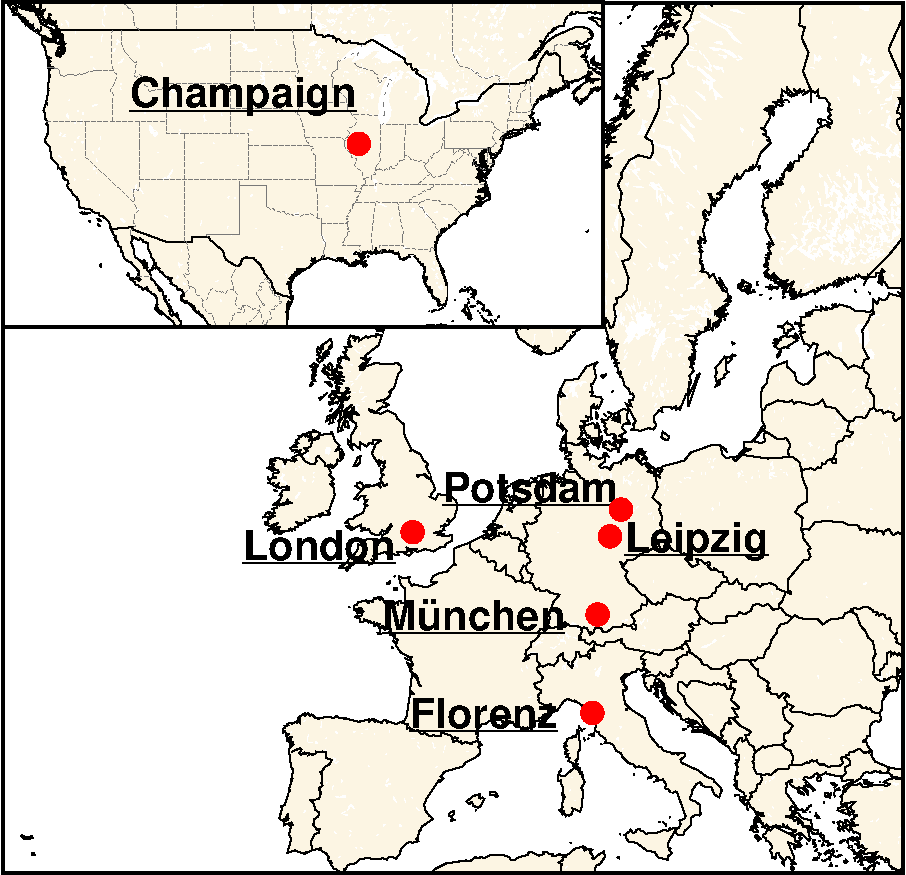
\includegraphics[scale=0.3]{../img/globalEXP.pdf}
	\vspace{2mm}
	\hrule
	\vspace{-3mm}
	\section*{\fontsize{18pt}{24pt}\selectfont \color{pblue} OS Erfahrung}
	\vspace{-2mm}
	\begin{itemize}
	\centering
	\item[\textbf{\LARGE \faLinux}]
\includegraphics[scale=0.50]{../img/5stars.png}\vspace{-2mm}
	\item[\textbf{\LARGE \faWindows}]
\includegraphics[scale=0.50]{../img/4stars.png}\vspace{-2mm}
    \item[\textbf{\LARGE \faApple}]
\includegraphics[scale=0.50]{../img/1stars.png}
    \end{itemize}
	\hrule
	\vspace{-2mm}
    \section*{\fontsize{18pt}{24pt}\selectfont \color{pblue} Programmierung}
	\vspace{-2mm}
	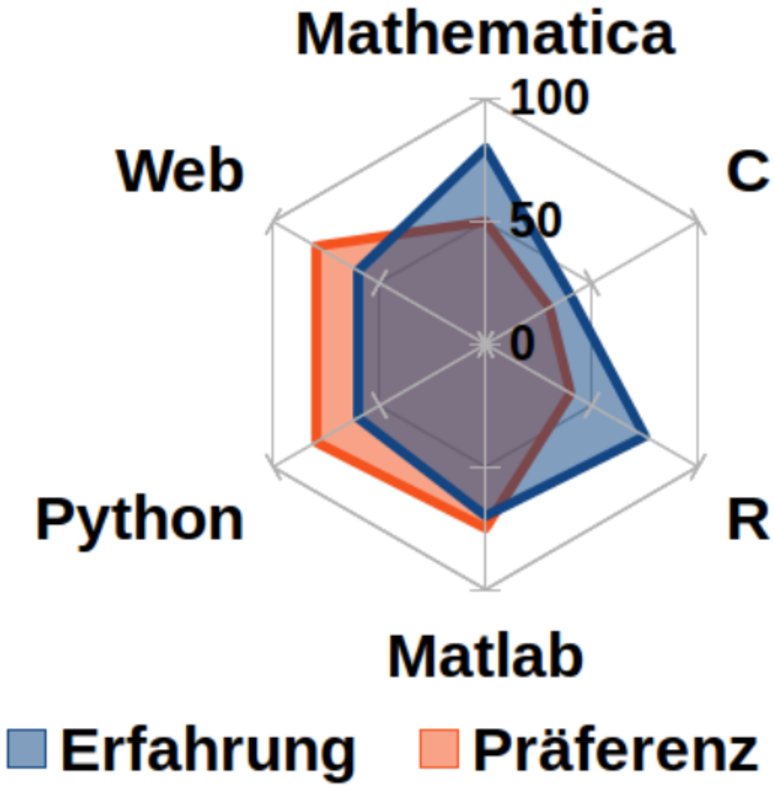
\includegraphics[scale=0.3]{../img/programmierung.pdf}
	\vspace{2mm}
	\hrule
	\vspace{-2mm}
	\section*{\fontsize{18pt}{24pt}\selectfont \color{pblue} Sprachen}
	\vspace{-2mm}
	\begin{itemize}
	\centering
	\item[\textbf{Deutsch}] 
\includegraphics[scale=0.50]{../img/5stars.png}\vspace{-2mm}
	\item[\textbf{Englisch}]  
\includegraphics[scale=0.50]{../img/4stars.png}\vspace{-2mm}
    \item[\textbf{Italienisch}] 
\includegraphics[scale=0.5]{../img/3stars.png}\vspace{-2mm}
    \item[\textbf{Französisch}]  
\includegraphics[scale=0.50]{../img/2stars.png}
    \end{itemize}
	\hrule
	\vspace{-2mm}
	 \section*{\fontsize{18pt}{24pt}\selectfont \color{pblue} Interessen}
	\vspace{-2mm}
	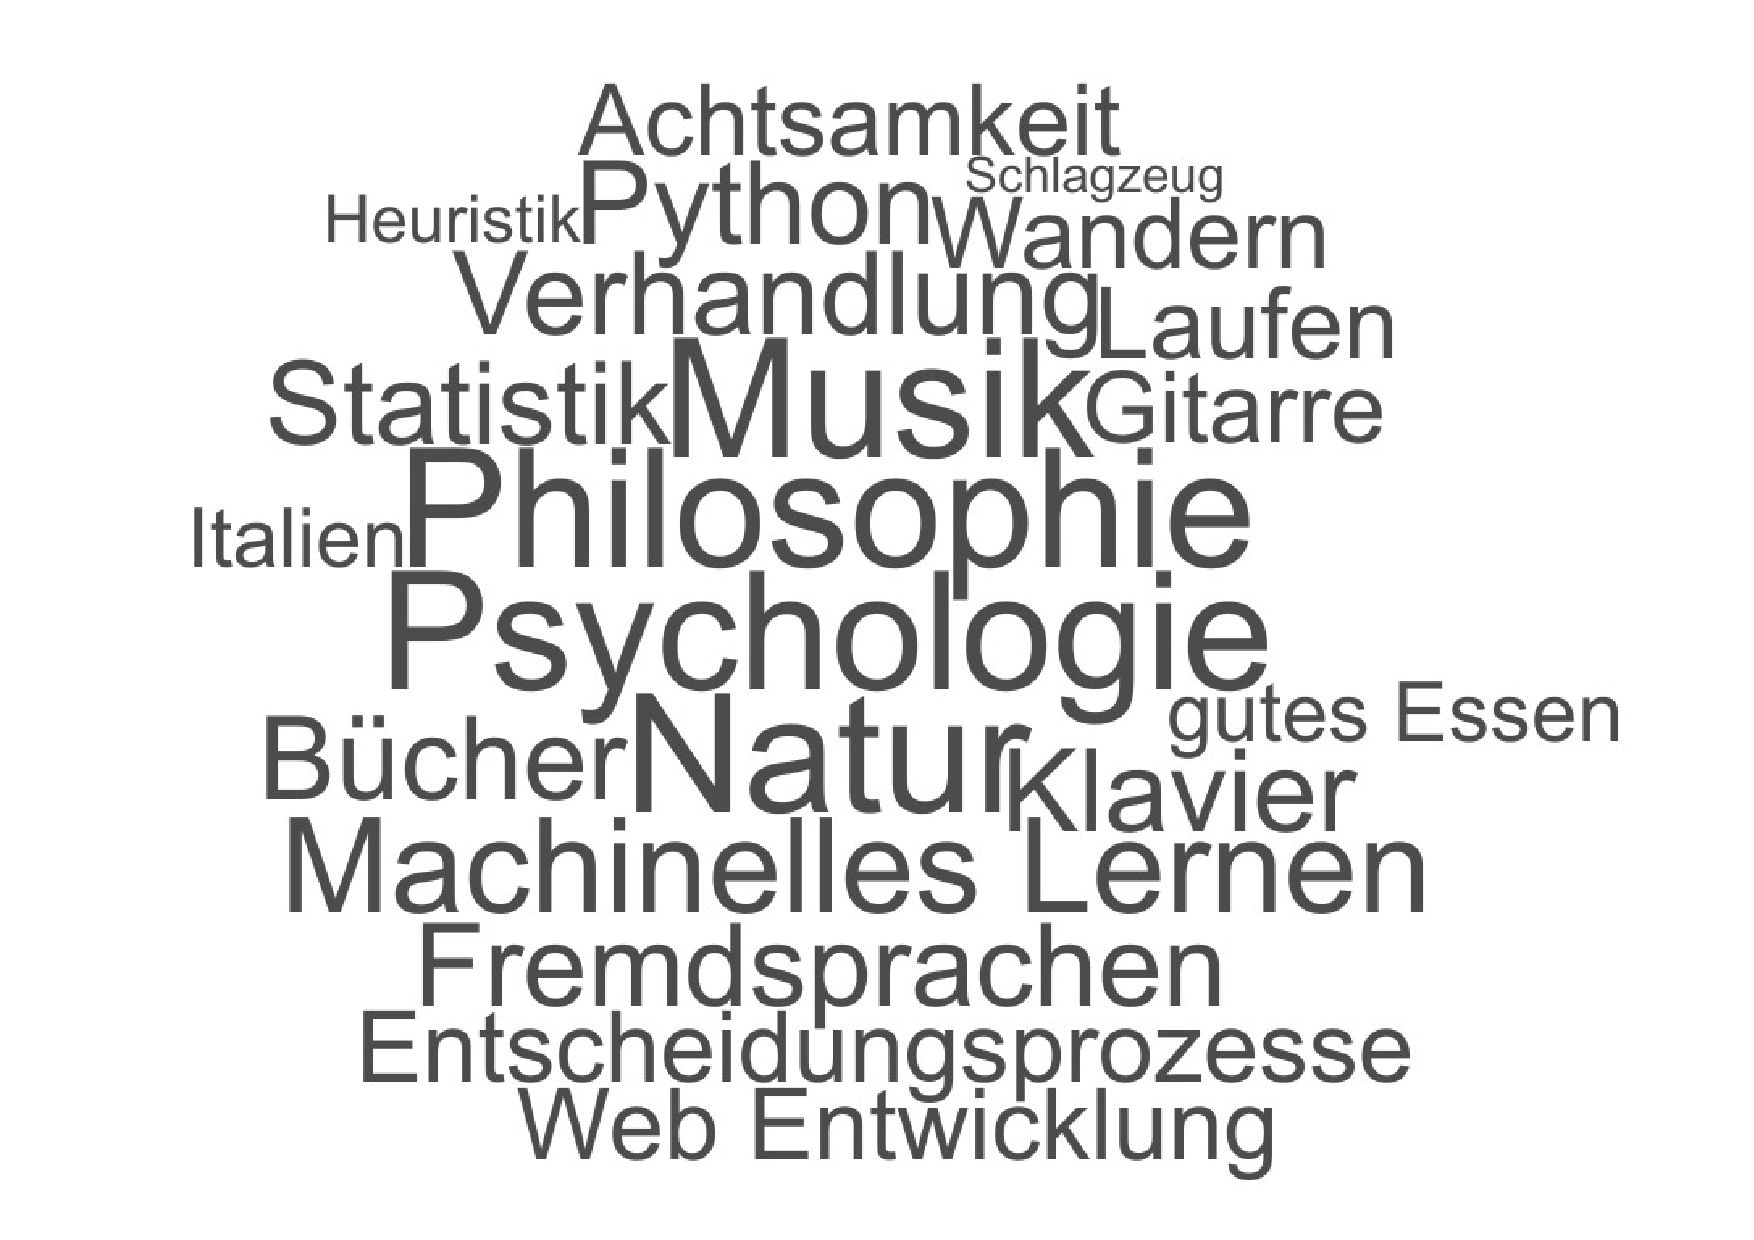
\includegraphics[trim=0cm 1cm 0cm 1cm, clip,scale=0.17]{../img/wordcloudGER.pdf}
\end{minipage}
\vrule
\hfill
\begin{minipage}[t]{0.67\textwidth}
		\section*{\fontsize{18pt}{24pt}\selectfont \color{pblue} Bildung}
		\begin{minipage}{0.34\textwidth}
	\textbf{\color{pblue}\faHourglassHalf~Master of Science} \\
	\textbf{Geowissenschaften}\\
	\textbf{\underline{Vertiefung:}~Geophysik}\\\\
	\textbf{\underline{Abschlussarbeit}}:\\
	\href{https://github.com/silvioschwarz/master-thesis}{Forecasting Macroseismic Intensities: A Sensitivity Study of a Bayesian Approach} (abgebrochen)\\\\\\
		10/2011 - aktuell\footnote{längere Pause auf Grund von Krankheit}\\
	Universität Potsdam
		\end{minipage}
		\hfill
		\begin{minipage}{0.3\textwidth}
		\vspace{-2mm}
	\textbf{\href{https://www.dropbox.com/s/297g1chiby8mrd3/Bachelor-Certificate.pdf?dl=0}{\color{pblue}\faGraduationCap~Bachelor of Science}}\\
	\textbf{Geowissenschaften}\\\\\\
	\textbf{\underline{Abschlussarbeit}}:\\
	\href{https://www.dropbox.com/s/3kngo4hpb0c47ww/Bachelorarbeit.pdf?dl=0}{\pdftooltip{Simulation von Bodenbewegungsszenarien von Starkbeben}{engl.: Simulating Ground Motion Scenarios of strong Earthquakes}}\\\\\\\\
	{10/2008 - 09/2011}\\
Universität Potsdam\\\\
		\end{minipage}
		\hfill
		\begin{minipage}{0.27\textwidth}
		\vspace{-2mm}
	\textbf{\href{https://www.dropbox.com/s/nsgmvy7o64xb9si/Abiturzeugnis.pdf?dl=0}{\color{pblue}\faGraduationCap~Abitur}}\\
	\textbf{Mathematik}\\
	\textbf{Geographie}\\\\
	\textbf{\underline{Abschlussarbeit}}:\\
	 \pdftooltip{Naturkatastrophen und ihr Einfluss auf das Leben in der Gegenwart}{engl.: Natural Disasters and their Impact on Life in the Present}\\\\\\\\
	 08/2000 - 05/2008\\
Klosterschule Roßleben (staatl. Gymnasium)\\
		\end{minipage}
		\hrule
		\section*{\fontsize{18pt}{24pt}\selectfont \color{pblue} Arbeitserfahrung}
		\begin{minipage}{0.49\textwidth}
		%\vspace{-60mm}
		\begin{minipage}[t]{0.25\textwidth}
		11/2017 - 03/2018\\ (5 Monate)
		\end{minipage}
		\hfill
		\begin{minipage}[t]{0.75\textwidth}
		\textbf{Werksstudent}\\ \href{https://assecor.de/}{\color{pblue}DB Dialog}\\
	    Unterstützung im Beschwerdemanagement
		\end{minipage}
		
		\vspace{0.5cm}
		
		\begin{minipage}[t]{0.25\textwidth}
		08/2014 - 06/2015\\ (11 Monate)
		\end{minipage}
		\hfill
		\begin{minipage}[t]{0.75\textwidth}
		\textbf{Werksstudent}\\
		\href{https://assecor.de/}{\color{pblue}Assecor GmbH}\\
	    Dokumentation des Stromnetzwerkes von Berlin, Deutschland für Vattenfall Europe Sales GmbH
		\end{minipage}
		
		\vspace{0.5cm}
		
		\begin{minipage}[t]{0.254\textwidth}
		11/2013 - 03/2014 \\ (5 Monate)
		\end{minipage}
		\hfill
		\begin{minipage}[t]{0.75\textwidth}
		\textbf{Werksstudent}\\
		\href{https://assecor.de/}{\color{pblue}Assecor GmbH}\\
	    Migration der IT Infrastruktur für\\ BIOTRONIK SE \& Co. KG
		\end{minipage}
		\\\\\\\\\\\\\\\\\\\\
		\end{minipage}	
		\hfill
		\vrule	
		\hfill
		\begin{minipage}{0.49\textwidth}
%		\begin{minipage}[t]{0.3\textwidth}
%		12/2017 - 03/2018\\ (4 Monate)
%		\end{minipage}
%		\hfill
%		\begin{minipage}[t]{0.7\textwidth}
%		\textbf{studentischer Assistent}\hfill \href{https://gfz-potsdam.de/}{\color{pblue}GFZ Potsdam}\\
%	    Sektion 2.4: Seismologie\\ automatisierte Qualitätskontrolle seismischer Stationen im AlpArray Netzwerk
%		\end{minipage}\vspace{0.5cm}
		\begin{minipage}[t]{0.25\textwidth}
		09/2012 - 11/2012 \\ (3 Monate)
		\end{minipage}		
		\hfill
		\begin{minipage}[t]{0.75\textwidth}
		\textbf{Master Praktikum}\\
		\href{https:///www.wolframalpha.com/}{\color{pblue}Wolfram$\mid$Alpha, IL, USA}\\
	    Entwicklung von geophysikalischen Inhalten für Wolfram$~\mid~$Alpha\hfill \href{https://m.wolframalpha.com/input/?i=moment+magnitude}{\color{pblue}Beispiel}\\
	    Betreuung: \href{mailto:bjornz@wolfram.com }{Dr. Björn Zimmermann} und \href{mailto:mtrott@wolfram.com }{Dr. Michael Trott} 
		\end{minipage}
		
		\vspace{0.5cm}
		
		\begin{minipage}[t]{0.25\textwidth}
		06/2011 - 08/2012 \\ (1 Jahr 3 Monate)
		\end{minipage}
		\hfill
		\begin{minipage}[t]{0.75\textwidth}
		\textbf{studentischer Assistent}\\
		\href{https://www.uni-potsdam.de/}{\color{pblue}Universität Potsdam}\\
	    Seismologische Modellentwicklung und Beratung für die Council for Geoscience, Pretoria, South Africa\\ Arbeitsgruppe \href{http://www.geo.uni-potsdam.de/mitarbeiterdetails/show/96/Frank_Scherbaum.html/}{\color{pblue}Prof. Frank Scherbaum}%\\
	    %1-wöchige Beratung am Imperial College London für \href{https://www.imperial.ac.uk/people/j.bommer}{\color{pblue}Prof. Julian J. Bommer} SSHAC LEVEL 3 PSHA
		\end{minipage}
		
		\vspace{0.5cm}
		
		\begin{minipage}[t]{0.25\textwidth}
		03/2011 - 04/2011 \\ (1 Monat)
		\end{minipage}		
		\hfill
		\begin{minipage}[t]{0.75\textwidth}
		\textbf{Bachelor Praktikum}\\
		\href{http://geologie.physgeo.uni-leipzig.de}{\color{pblue}Universität Leipzig}\\
	    Wartung des sächsischen seismologischen Netzwerks\\ Betreuung: \href{mailto:sfunke@rz.uni-leipzig.de}{Dipl. Geophys. S. Funke}
		\end{minipage}
		
		\vspace{0.5cm}
		
%		\begin{minipage}[t]{0.25\textwidth}
%		03/2010 - 05/2010 \\ (3 Monate)
%		\end{minipage}
%		\hfill
%		\begin{minipage}[t]{0.75\textwidth}
%		\textbf{studentischer Assistent}\\
%		\href{https://www.uni-potsdam.de/}{\color{pblue}Universität Potsdam}\\
%	    Qualitätskontrolle von Algorithmen im Rahmen seismischer Gefährdungsanalyse\\
%	    Arbeitsgruppe \href{http://www.geo.uni-potsdam.de/mitarbeiterdetails/show/96/Frank_Scherbaum.html}{\color{pblue}Prof. Frank Scherbaum}\	    
%		\end{minipage}
		\end{minipage}
		\hrule
		\section*{\fontsize{18pt}{24pt}\selectfont \color{pblue} Projekte}
		\begin{itemize}
		\item TerremotoPi \href{https://github.com/silvioschwarz/TerremotoPi}{
\includegraphics[scale=0.05]{../img/terremotoPiIcon.png}}
		\item Eathquake Distances \href{https://github.com/silvioschwarz/Earthquake-Distances}{\faGithub}
		\end{itemize}
\end{minipage}
\end{document}